\chapter{Design and Implementation}\label{chp:designimpl}
This chapter suggests a prototype implementation of one possible application, on background of the principles and ideas in the previous two sections. The protocol structure will be displayed, together with examples from the code and test runs using the system.

\section{System specifications}\label{sec:chat}
As mentioned in \ref{sec:apps} there are several scenarios where functional key exchange can provide security and privacy. This section will describe the structure and specifications for a chat system utilizing \gls{abake} as described in \ref{sec:abake} and \cite{DBLP:abake}. The system consists of a set of clients running a client application and a broadcast server. It could easily have been altered to support peer-to-peer, since the server only acts as a intermediate for broadcasting, caching of encapsulations and policy management. The system shown is meant to be a proof of concept for how this kind of application could look, it is thus simplified to some extent. Most of the data used are static to abstract away difficulties with administration of rooms and related policies, as well as key management. The implementation will not address key distribution, therefor a key is given to the users on connection. The extended system would include a separate \gls{kms} which the users would register with to obtain their key. The best solution would probably be to have a separate virtual or physical server doing each task; attribute and key management, storage and distribution of keying material, broadcasting of chat messages/cipher texts. Other features like being able to create your own rooms and administrate these would also be logical. This prototype will be a single room with a static policy.
\paragraph{The most important feature} of the system is to provide encrypted communication between users whom satisfy the room policy. The users should obtain a shared session key through \gls{abake}. This way we assure implicit authentication of all users taking part in the conversation. A user should be able to participate in the exchange without ever having to provide an identity. It is assumed that all users have registered with some \gls{kms} prior to the key exchange, a user would typically register a set of attributes which would have to be approved by the system authority. When new users join, they should be able to upload their contribution and receive the rest of the keying material from the server; the users will then have to compute the new session key. After exchanging keys, the users should be able to use it to encrypt the chat messages. It should be noted that anybody can in fact upload a contribution and receive encapsulations, but only the ones with the correct attributes can decapsulate and produce the session key. It might be smart for the server to challenge the new user to prove that he has the correct attributes. The server could require that new users prove that they have the correct attributes before being able to upload, to avoid denial of service attacks on the communication channel. This extension would simply mean the server challenging the new user with a encrypted nonce which the user would have to encrypt and send back. This mechanism was not included in this implementation as as this project focus on demonstrating the key exchange process, and since this possible weakness not pose any threats to the integrity of the system it is not prioritized. 


\section{Models and construction}
The high level construction of the key exchange used in the system is based on the generic one-round AB-AKE protocol presented by Gorantal et al. \cite{gorantla2010attribute}. The main differences being the encapsulation function used, the implementation described in this project is constructed based on the \gls{abe} scheme implemented in Charm, as described in \ref{subsec:ABE} and \cite{abe_waters09}, while \cite{gorantla2010attribute} introduce \gls{epabkem}. This project propose a complete system utilizing the key exchange, so after obtaining a shared key, users encrypt their messages using a standard symmetric key encryption algorithm. The messages are broadcast through the same broadcast server used for key exchange. When a new user joins, the message exchanges are paused until the new key is calculated by all users. Figure \ref{fig:flow} shows the system flow when a new user connects. A client will first query the server for the room policy, before a encapsulation is generated from the received policy. This one is sent to the server which distributes it so that all users have all contributions. After doing this distribution, the server will go back to being a pure broadcast server for chat messages. Figure \ref{fig:encapdistr} illustrates the encapsulation distribution process. Bob is a new user, so he uploads his contribution to the server, there are $n$ users already in the system. Next the server broadcast Bob's encapsulation to the current users, before sending the set of active encapsulations to Bob. After obtaining all encapsulations, all users initiate the key generation procedure, as shown in figure \ref{fig:keygen}, which consist of decapsulating the encapsulations, then using the symmetric keys with a pseudo random function on a session id, before combining them using bitwise xor. For the pseudo random function keyed hmac from the python library is used. The session id is the concatenation of the socket addresses of each user, as for the presented implementation these addresses are sent from the server together with the encapsulations, but if the system was to be extended to a peer-to-peer configuration, each encapsulation would be sent individually from different addresses and could then be obtained by the users directly. 




\begin{figure}[H]
\begin{mdframed}
Let $U_i = \{u_1,u_2,\dots,u_n\}$ be the set of users participating in the key exchange. $Sk_i$ is the corresponding user's secret keys. $C_j = c_1,c_2,\dots,c_n$ is the set of encapsulations. $A_j$ is the network address of each user.
\paragraph{Decapsulation} - $k_j$ is the symmetric key of encapsulation $c_j$. Each user, $u_i$, decapsulates all encapsulations as follows.
\centerline{For $j\neq i \hspace{1cm}   k_j \leftarrow Decapsulate(Sk_i, C_j)$}

\paragraph{Session id} - $Sid = A_1 \parallel A_2 \parallel \dots \parallel A_n$
\paragraph{Session key computation} - $K = {hmac_k}_1(Sid) \oplus \dots \oplus {hmac_k}_n(Sid)$

\caption{Key generation procedure}\label{fig:keygen}
\end{mdframed}
\end{figure}

\paragraph{Security concerns}
The focus is on the security of the session keys used to secure the communication and because these are generated from the encapsulations of the users it makes sense to consider both security of the generated session key and the encapsulations. Notions of forward and backwards secrecy is used differently according to the context, where the original definition assume a long-term key with a session key established using this and that future exposure of the long-term key would not reveal the session key. Alzaid et al. \cite{Alzaid2010} discuss how this is not always how the term is used, and that the current use in the context of group key communication is that a session key should not be revealed by compromisation of older keys. As for this system, it cannot be said that the key exchange itself is forward secure, since a user with the correct attributes can obtain all previous session keys by decapsulating and combining the correct set of encapsulations. What is forward secure though is the session key itself, meaning that if an old session key was to be lost, it would not affect the current session key. New session keys are calculated every time a new user joins, the users can be sure of this since they actually provide parts of the key material themself, this ensures forward secrecy in terms of the session key. This property is important because without it a new user could never be sure that a previous key might be compromised and reveal all the messages encrypted by him. This is especially important since new keys are generated all the time, by users joining, so that there will exist a lot of old session keys for each room. As for users leaving a decision was made not to generate new keys when users leave. If users trusted all the users currently in a room, the removal of one of these would not change the trust, and no new key needs to be generated, saving time and resources. Especially since the system presented here use only one server doing all the work, it is good to generate new keys as infrequently as possible, since the communication is paused during key exchange. The logical way of improving this would be to do the key exchange in parallel and start using the new key when the exchange is done. In this case some might also argue that creating a new session key on user leave would also be preferable.
In addition to this does much of the security of the system rely on the \gls{kms} not going rogue, but in the applications discussed, we can assume that the users trust the \gls{kms}, this is reasonable since each system or domain, would require users to register and thus agree to the terms and conditions of the system.



\begin{figure}[H]
\centering
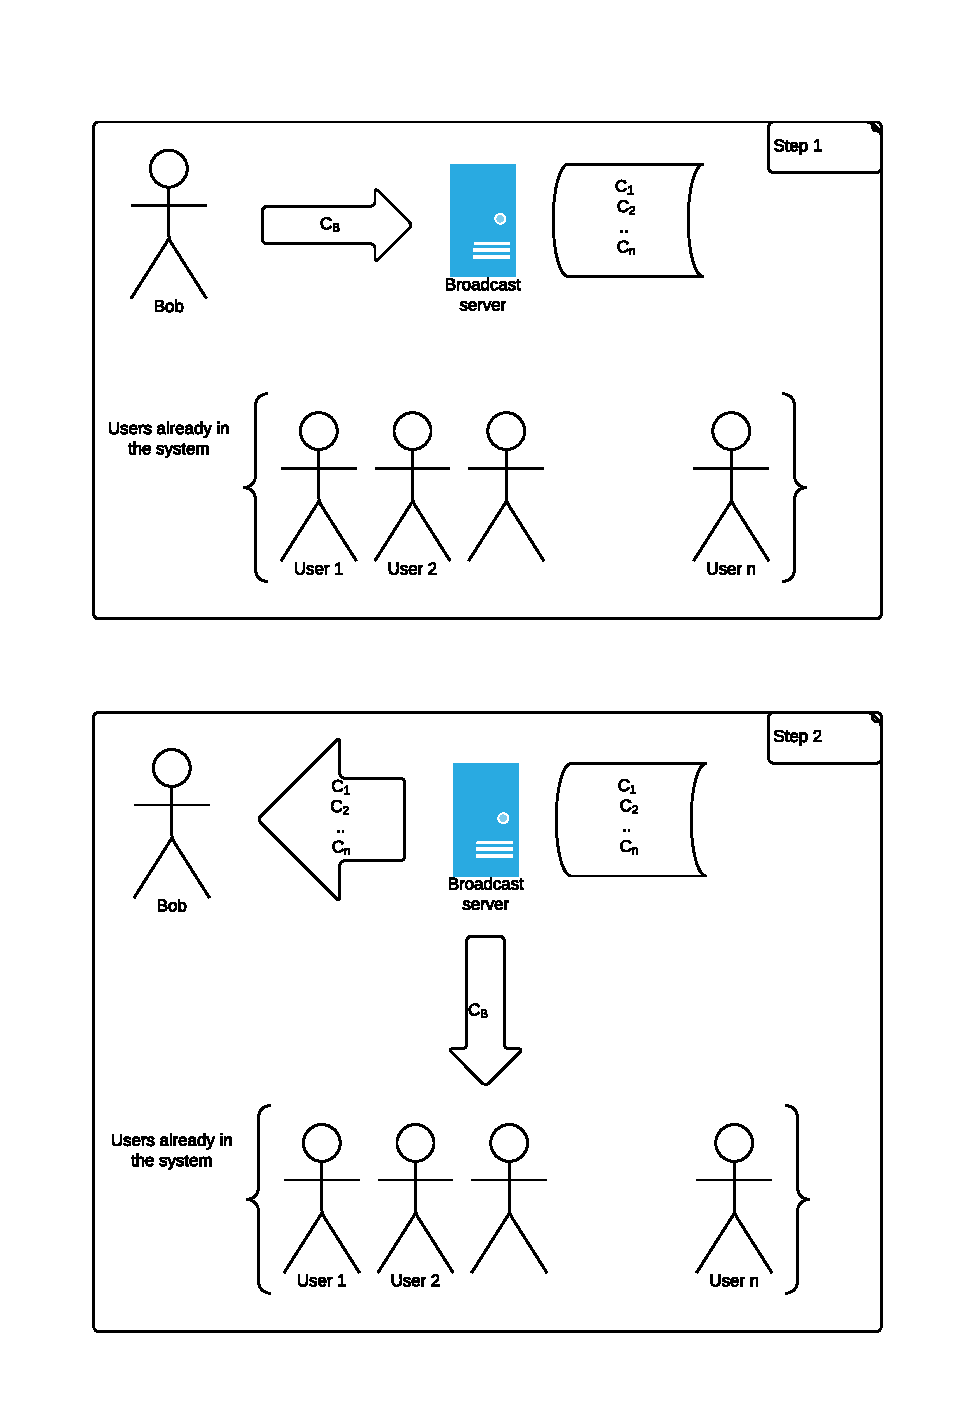
\includegraphics[trim=2cm 1.5cm 2cm 4cm ,scale=1]{chatsystem.pdf}
\caption{Distribution of encapsulations}
\label{fig:encapdistr}
\end{figure}

\begin{figure}[H]
\centering
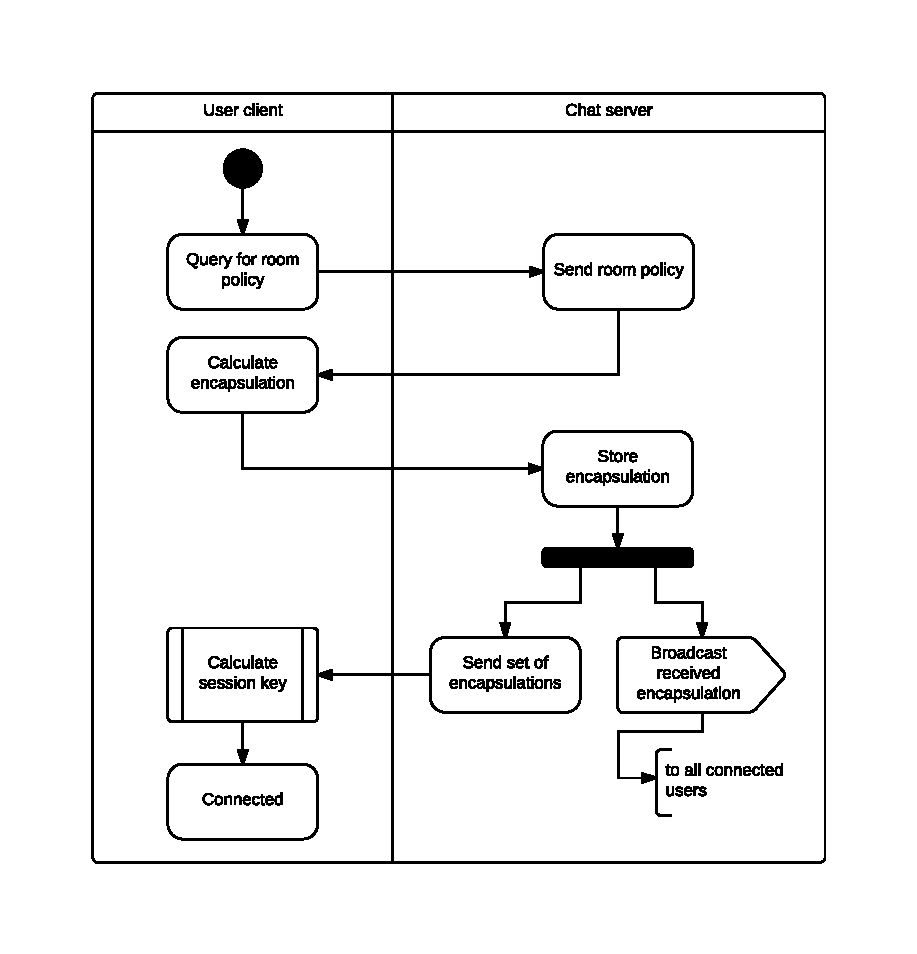
\includegraphics[trim=2cm 2cm 0cm 1cm ,scale=1]{Flow.pdf}
\caption{System flow.}
\label{fig:flow}
\end{figure}


\newpage

\section{Implementation}
The application will consist of to components, one server class and one client class. The implementations of these follow the state diagrams \ref{fig:server-state} and \ref{fig:client-state} respectively. This section will describe how these two classes are implemented, the complete implementation including the code is attached in appendix \ref{clientcode} and \ref{servercode}. The state diagrams represents exactly how the programs work together, the send and receive actions in the diagram represent sockets in the application, and the loop binding it together is equal to the main loops of each class. This eventually mean that a send in the figure have a corresponding socket.send() in the code.

\begin{figure}
\centering
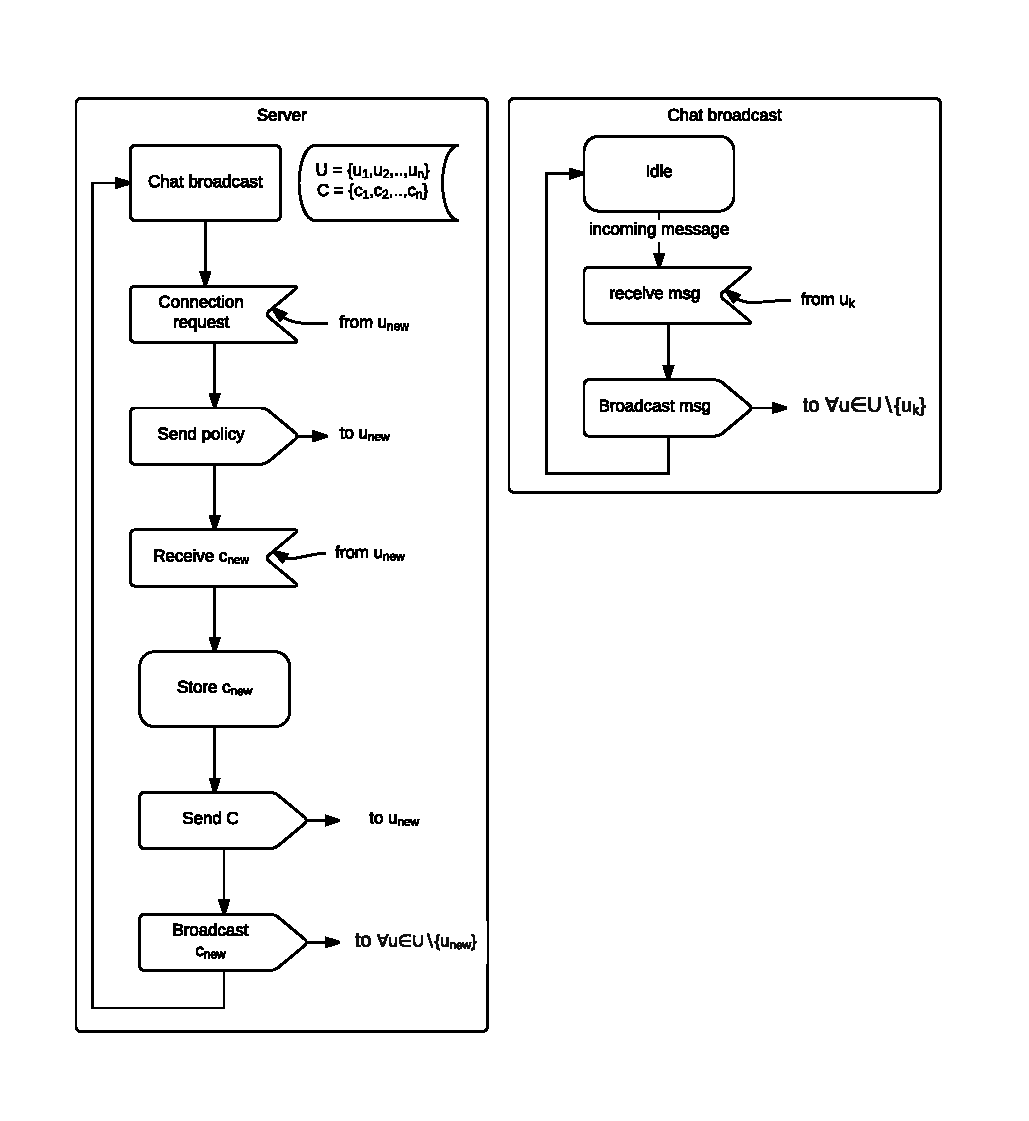
\includegraphics[trim=2cm 1.5cm 2cm 4cm ,scale=1]{server-state.pdf}
\caption{Internal flow of the server class}
\label{fig:server-state}
\end{figure}


\begin{figure}
\centering
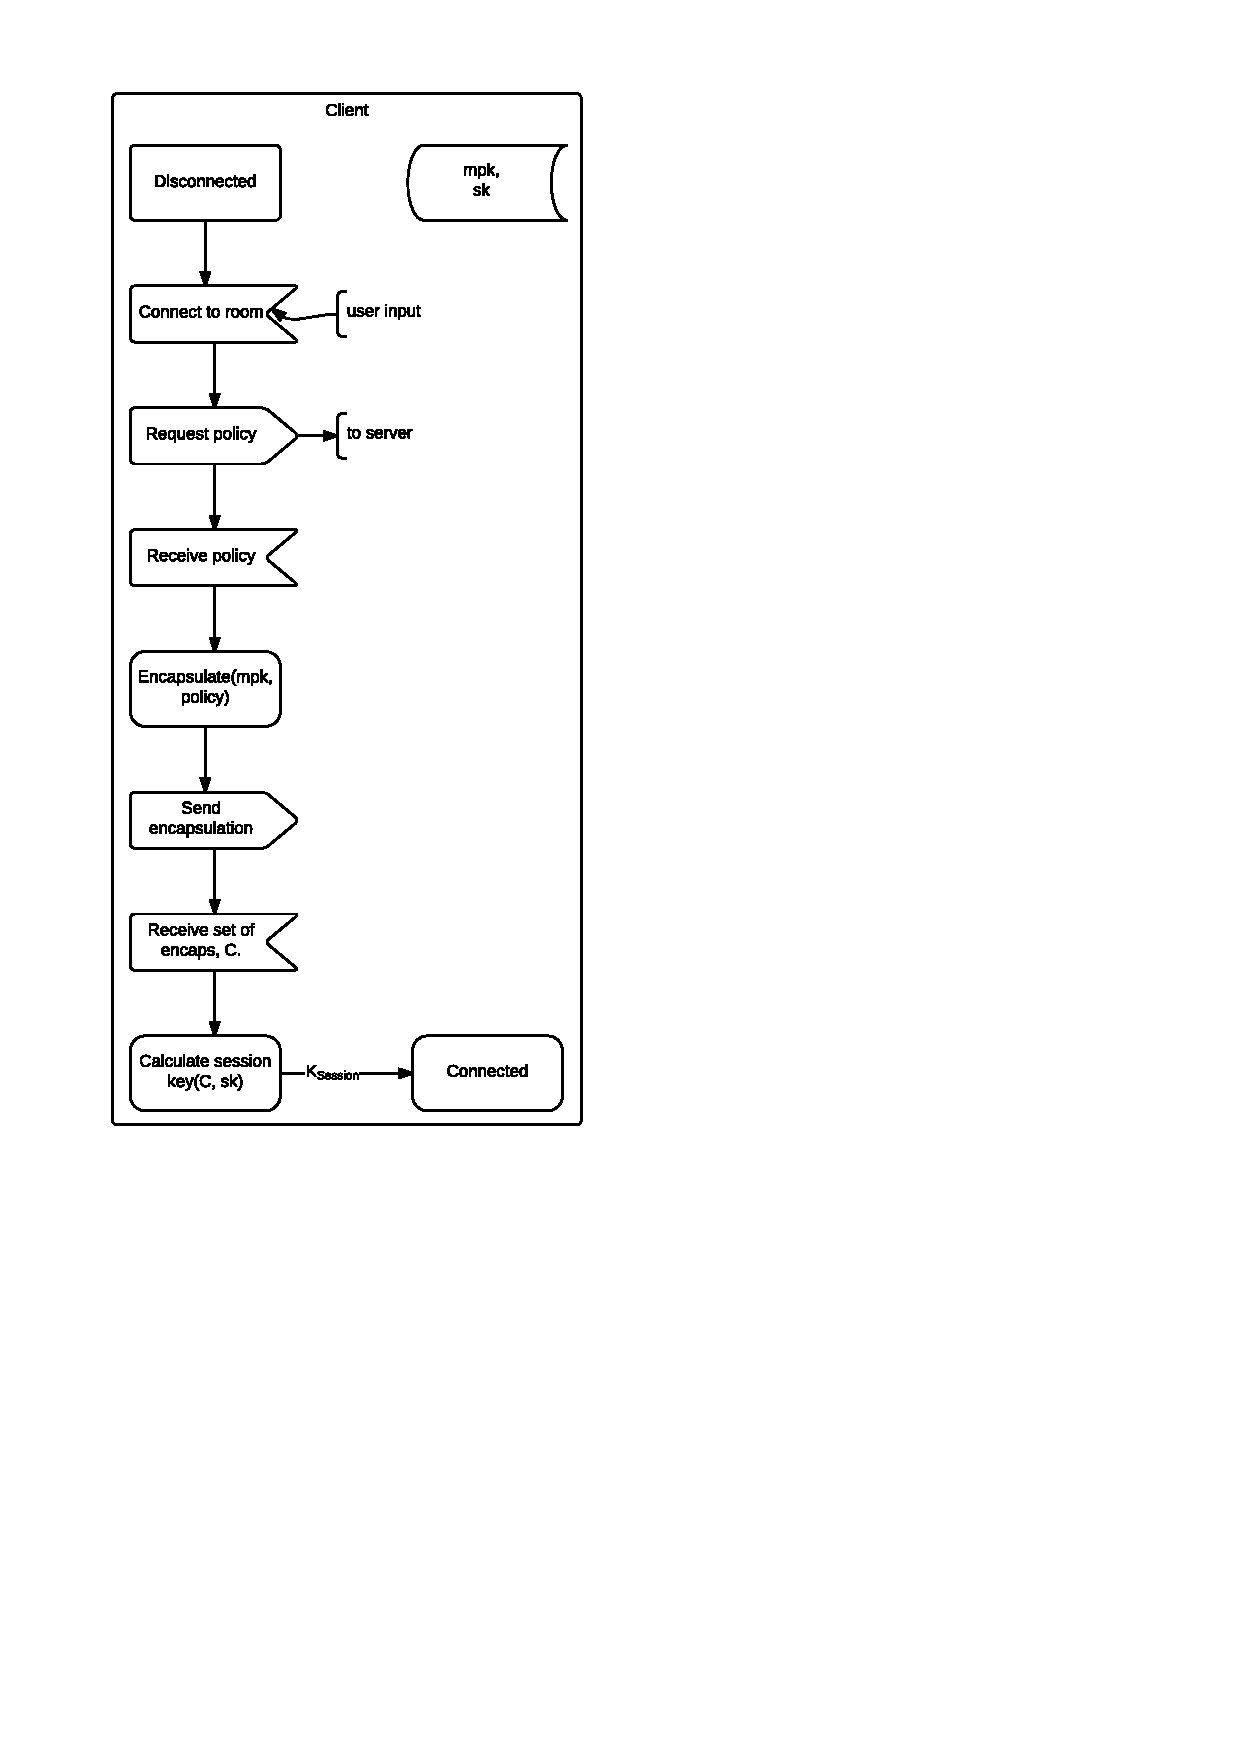
\includegraphics[trim=0cm 11cm 0cm 0cm, scale=1]{client-state.pdf}
\caption{Internal flow of the client class}
\label{fig:client-state}
\end{figure}

\section{System demonstration}
This section will try to demonstrate how the system looks in practice, figure \ref{fig:server-output} and \ref{fig:client12-output} shows how the system acts from the perspective of the server and from the clients, respectively. First the server is started with a preset policy as highlighted in \ref{fig:server-output}, then two users join in succession, it can be seen that for each new user encapsulations are broadcast. The clients that connect can be observed in \ref{fig:client12-output} - when starting the client program, it will automatically try connecting to the server on address given as argument to the program. After connecting, the server will start by sending the room policy and setup the user with a attribute key and the public parameters, as discussed earlier this is done to abstract away the problem of key distribution. It would also be more complicated to keep the keys persistent, since it would have to be stored somewhere locally, on a deployed system these keys would be in the user data of each registered user. After receiving the policy, the client uploads his encapsulation and we can see that he receives the current set from the server - which in the case of one user only is his own, which he already have. When the second user joins it can be seen that the first user generates a new key which is the same as the one generated at the second user. The messages are now encrypted using this key.
\begin{figure}
\centering
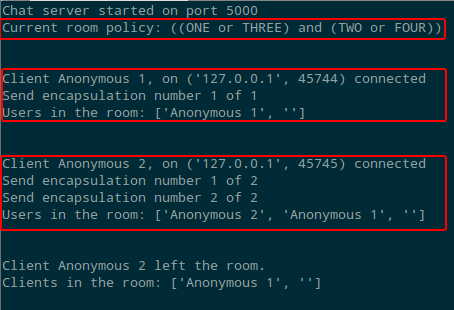
\includegraphics[width=\linewidth]{server.png}
\caption{Server output}
\label{fig:server-output}
\end{figure}

\begin{figure}
\centering
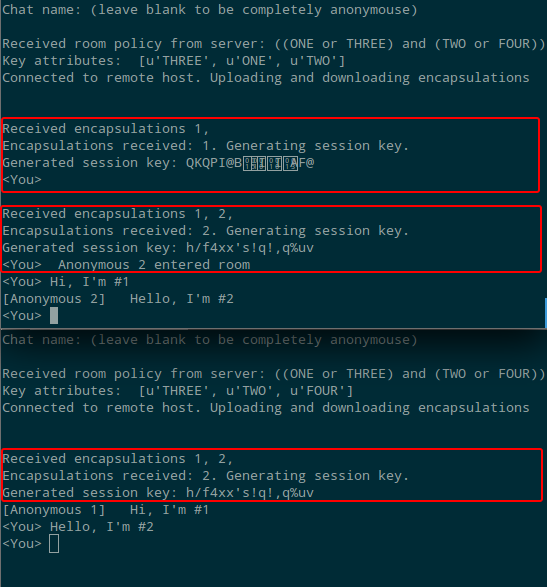
\includegraphics[width=\linewidth]{client1and2.png}
\caption{Client 1 and 2 output}
\label{fig:client12-output}
\end{figure}
